\chapter{Proposta}

Conforme apresentado nos capítulos anteriores, a modelagem de um sistema de detecção de fraude com a utilização de técnicas inspiradas no sistema imunológico natural oferece diversas vantagens. Esse trabalho busca identificar exatamente \emph{quanto} esses modelos podem aperfeiçoar os métodos existentes. O método utilizado é a comparação dos resultados da classificação de algoritmos tradicionais e Sistemas Imunológicos Artificiais sobre um mesmo conjunto de dados. Esta seção apresenta os elementos principais para o desenvolvimento da proposta.

\section{Descrição geral}

Os principais elementos no desenvolvimento do trabalho são: os conjuntos de dados utilizados na execução dos testes, os algoritmos que serão testados nesses dados e os métodos de avliação dos resultados.

\subsection{Descrição dos dados}

Para os testes, serão utilizados dois conjuntos de dados contendo informações de contas de cartões de crédito. Esses dados estão disponíveis publicamente e fazem parte de um projeto chamado StatLog. Esse projeto foi concebido para testar diversos métodos de classificação em problemas grandes e comercialmente relevantes, comparando os resultados e determinando o quanto essas diferentes técnicas atendiam as necessidades da indústria. Conforme a própria descrição do projeto, os objetivos do projeto eram três:

\begin{enumerate}[a)]
    \item Possibilitar medidas críticas de desempenho para procedimentos de classificação disponíveis,
    \item Indicar a natureza e escopo dos desenvolvimentos futuros necessários para que os métodos atendam as necessidades e expectativas dos usuários e
    \item Indicar as direções mais promissoras de desenvolvimento para abordagens comercialmente imaturas.
\end{enumerate}

Os conjuntos de dados são denominados German Credit (Cr.Ger) e Australian Credit (Cr.Aust). Ambos contém informações sobre contas de crédito, conforme apresentado nas próximas seções.

\subsubsection{Cr.Ger}

Esse conjunto de dados foi cedido pelo professor Hans Hoffman, da Universidade de Hamburgo. Os atributos e valores que esses atrbutos podem são descritos na listagem \ref{lst:ge_dataset} \footnote{Na descrição dos atributos, DM significa \emph{deutsche mark} (marco alemão), a moeda corrente na Alemanha na época da coleta dos dados. Para efeito de comparação, o Banco Central Europeu estipulou a conversão irrevogável do marco alemão, a partir de 1º de janeiro de 1999, em DM 1.95583 = \euro 1 (http://www.ecb.int/press/pr/date/1998/html/pr981231\textunderscore2.en.html).}.

\begin{lstlisting}[caption=Atributos do conjunto de dados alemão,label=lst:ge_dataset]
    Atributo 1: (qualitativo)
    Situação da conta corrente existente
    A11 : ... < 0 DM
    A12 : 0 <= ... < 200 DM
    A13 : ... >= 200 DM
    A14 : sem conta corrente

    Atributo 2: (numérico)
    Duração em meses

    Atributo 3: (qualitativo)
    Histórico de crédito
    A30 : nenhum crédito retirado / todos os créditos pagos apropriadamente
    A31 : todos os créditos nesse banco pagos apropriadamente
    A32 : créditos existentes pagos apropriadamente até agora
    A33 : atraso no pagamento no passado
    A34 : conta crítica / outros créditos existentes (não nesse banco)

    Atributo 4: (qualitativo)
    Propósito
    A40 : carro (novo)
    A41 : carro (usado)
    A42 : móveis/equipamento
    A43 : rádio/televisão
    A44 : eletrodomésico
    A45 : reparos
    A46 : educação
    A47 : (férias - não existe no conjunto de dados)
    A48 : reciclagem profissional
    A49 : negócios
    A410 : outros

    Atributo 5: (numérico)
    Quantidade de crédito

    Atributo 6: (qualitativo)
    Poupança
    A61 : ... < 100 DM
    A62 : 100 <= ... < 500 DM
    A63 : 500 <= ... < 1000 DM
    A64 : .. >= 1000 DM
    A65 : desconhecido / sem poupança

    Atributo 7: (qualitativo)
    Emprego atual desde
    A71 : desempregado
    A72 : ... < 1 ano
    A73 : 1 <= ... < 4 anos
    A74 : 4 <= ... < 7 anos
    A75 : .. >= 7 anos

    Atributo 8: (numérico)
    Taxa de parcelamento em porcentagem do rendimento disponível

    Atributo 9: (qualitativo)
    Estado civil e sexo
    A91 : masculino : divorciado/separado
    A92 : feminino : divorciada/separada/casada
    A93 : masculino : solteiro
    A94 : masculino : casado/viúvo
    A95 : feminino : solteira

    Atributo 10: (qualitativo)
    Outros devedores / fiadores
    A101 : nenhum
    A102 : devedor solidário
    A103 : fiador

    Atributo 11: (numérico)
    Residência atual desde

    Atributo 12: (qualitativo)
    Propriedade
    A121 : imóvel
    A122 : se não A121 : financiamento / seguro de vida
    A123 : se não A121/A122 : carro ou outro, não incluso no atributo 6
    A124 : desconhecido / sem propriedade

    Atributo 13: (numérico)
    Idade em anos

    Atributo 14: (qualitativo)
    Outros planos de parcelamento
    A141 : banco
    A142 : lojas
    A143 : nenhum

    Atributo 15: (qualitativo)
    Residência
    A151 : alugada
    A152 : própria
    A153 : gratuita

    Atributo 16: (numérico)
    Número de créditos existentes nesse banco

    Atributo 17: (qualitativo)
    Emprego
    A171 : desempregado / sem proficiência / não-doméstico
    A172 : sem proficiência / doméstico
    A173 : proficiente / funcionário público
    A174 : administrador / auto-empregado /
           empregado altamente qualificado / oficial

    Atributo 18: (numérico)
    Número de dependentes

    Atributo 19: (qualitativo)
    Telefone
    A191 : nenhum
    A192 : sim, registrado sob o nom do consumidor

    Atributo 20: (qualitativo)
    Trabalhador estrangeiro
    A201 : sim
    A202 : não
\end{lstlisting}

\subsubsection{Cr.Aust}

Os atributos do conjunto de dados australiano são descritos na listagem \ref{lst:au_dataset}. Uma grande desvantagem, muito comum nesse tipo de conjunto de dados (seção \ref{fraud:data}), é a de o nome dos campos ter sido alterado, perdendo o significado original.

\begin{lstlisting}[caption=Atributos do conjunto de dados australiano ,label=lst:au_dataset]
A1: b, a
A2: contínuo
A3: contínuo
A4: u, y, l, t
A5: g, p, gg
A6: c, d, cc, i, j, k, m, r, q, w, x, e, aa, ff
A7: v, h, bb, j, n, z, dd, ff, o
A8: contínuo
A9: t, f
A10: t, f
A11: contínuo
A12: t, f
A13: g, p, s
A14: contínuo
A15: contínuo
A16: +,- (atributo de classe)
\end{lstlisting}

\subsection{Algoritmos}

Os algoritmos que serão utilizados para a comparação são um pacote de algoritmos desenvolvido por Jason Brownlee \cite{Brownlee2007}. Esse pacote foi especialmente desenvolvido para a plataforma de aprendizagem de máquina Weka (descrita na seção \ref{sec:prop_weka}) e são disponibilizados através de uma liceça aberta (GNU GPL). Nele, são implementados diversos algoritmos de redes imunológicas e sistemas imunológicos artificiais, conforme a listagem abaixo:

\begin{enumerate}[a)]
    \item \textbf{Learning Vector Quantization (LVQ)}: similar às redes neurais, que utiliza aprendizagem supervisionada, baseada em protótipos, para classificação de dados. É similar ao algoritmo de k-vizinhos mais próximos e um precursor do próximo algoritmo.
    \item \textbf{Self-Organizing Map (SOM)}: algoritmo de redes neurais que utiliza aprendizagem não-supervisionada. Mapeia os valores da base de dados produzindo um mapa: um espaço de duas dimensões, uma representação discreta dos dados de entrada.
    \item \textbf{Feed-Forward Artificial Neural Network (FF-ANN)}: tipo de algoritmo de redes neurais onde o sinal é propagado na direção entrada-saída, sem conexões de \emph{feedback}.
    \item \textbf{Artificial Immune Recognition System (AIRS)}: algoritmo imunológico supervisionado descrito na seção \ref{sec:prop_airs}.
    \item \textbf{Clonal Selection Algorithm (CLONALG)}: um dos principais algoritmos imunológicos, descrito na seção \ref{sec:ais_clonalg}.
    \item \textbf{Immunos-81}: algoritmo imunológico descrito na seção \ref{sec:prop_immunos}.
\end{enumerate}

\subsubsection{AIRS}
\label{sec:prop_airs}

Esse algoritmo foi criado por Andrew Watkins \cite{Andrew2003}. Ele tinha como objetivo implementar um Sistema Imunológico Artificial que utilizasse aprendizagem supervisionada, já que, na época de seu desenvolvimento, a área de algoritmos imunológicos supervisionados não havia sido explorada, apesar da pesquisa intensa na área de algoritmos imunológicos não-supervisionados \footnote{De acordo com o autor, o único outro algoritmo imunológico supervisionado era o Immunos, apresentado na próxima seção.}

Por esse motivo, esse foi o primeiro algoritmo supervisionado a implementar a maior parte das técnicas inspiradas nos sistemas imunológicos, como: modelagem dos dados como antígenos e anticorpos, expansão clonal dos linfócitos, mutação e maturação de afinidade e memória imunológica.

Na definição desse algoritmo, também foi aplicado o formalismo do espaço de formas. Conforme apresentado na seção \ref{sec:ais_shape}, esse é um formalismo bastante apropriado para a modelagem de Sistemas Imunológicos Artificiais, devido a forte semelhança entre o espaço de formas e as diferentes formas que os receptores dos linfócitos no sistema imunológico apresentam. Os antígenos identificados por esses receptores formam a região de reconhecimento ao redor de cada ponto no espaço de formas. Em um algoritmo de aprendizagem, isso representa a correspondência entre as instâncias de treinamento (antígenos) e as possíveis soluções (células B).

\subsubsection{Immunos}
\label{sec:prop_immunos}

Esse algoritmo foi apresentado por Jerome Carter \cite{Carter2000}. O algoritmo Imunnos foi desenvolvido em oposição aos algoritmos que tentavam simular fielmente o comportamento do sistema imunológico. Segundo o autor, do ponto de vista da computação, construir sistema que utilize equações cuidadosamente derivadas dos estudos teóricos a imunologia seria um feito notável, mas não ideal. Os elementos do sistema imunológico foram reduzidos ao nível mais fundamental para que fossem introduzidos no sistema.

O principal elemento na modelagem do algoritmo foi a utilização de pequenas e simples unidades de processamento conectadas em paralelo das redes neurais e linfócitos do sistema imunológico. As principais metas da modelagem eram:

\vspace{2mm}
\begin{enumerate}[a)]
    \itemsep1pt
    \item Representação interna simples de ser entendida,
    \item Capacidade de generalização sobre os dados de entrada,
    \item Tempos de treinamento previsíveis,
    \item Aprendizagem \emph{online},
    \item Potencial para atuar como memória associativa,
    \item Suporte a atributos contínuos e qualitativos,
    \item Capacidade de aprendizagem e recuperação de um grande número de padrões,
    \item Aprendizagem baseada em experiência e
    \item Aprendizagem supervisionada.
\end{enumerate}
\vspace{2mm}

\subsection{Weka}{}
\label{sec:prop_weka}

Como plataforma de testes, será utilizado o \emph{software} Weka. Weka (\emph{Waikato Environment for Knowledge Analysis}, Ambiente para Aprendizagem de Máquina de Waikato) é uma suite de aplicações de aprendizagem de máquina, desenvolvida na Universidade de Waikato, na Nova Zelândia. Essa ferramenta é largamente utilizada em projetos nessa área, devido a sua licença aberta (GNU GPL), que permite que seja utilizada quase sem restrições.

A figura \ref{fig:prop_weka} mostra uma captura de tela do programa em execução, mostrando a visualização do conjunto de dados alemão.

\begin{figure}[h!]
\centering
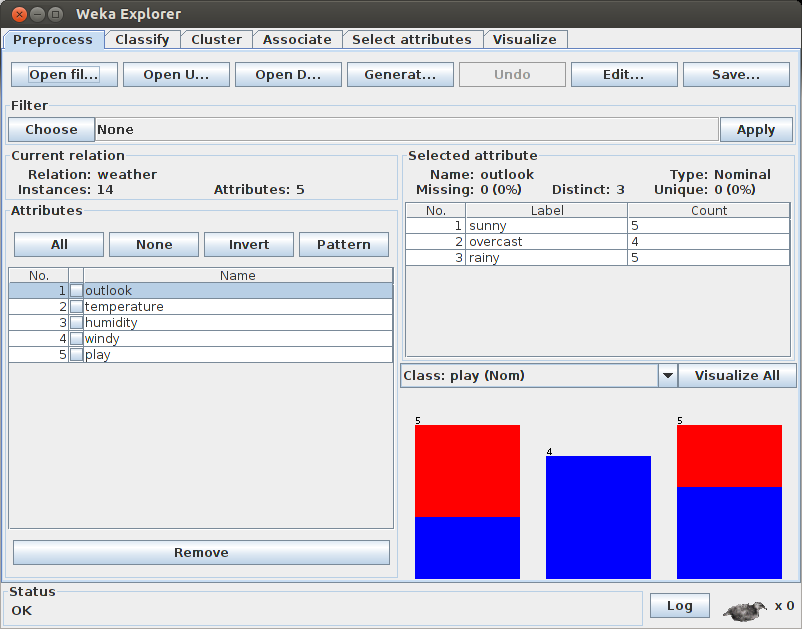
\includegraphics[width=0.75\textwidth]{img/weka.png}
\caption{Janela do módulo Explorer - Weka 3.6.4}
\label{fig:prop_weka}
\end{figure}

\iffalse arff file format \fi

\section{Arquitetura}

\section{Critérios}

Uma consideração importante quando analisa-se o desempenho de dois ou mais sistemas é que muito difícil (ou até mesmo impossível) excluir-se todos os fatores externos, resultando em uma análise completamente imparcial. Nesse caso específico, o resultado dos testes em cada algoritmo é fortemente influenciado pelas características dos dados na base de dados, embora os métodos de análise dos resultados procuram minimizar essa influência (conforme apresentado na seção \ref{sec:fraud_criteria}).

\section{Resultados}

\iffalse

\chapter{Conclusão}

\section{Síntese}

\section{TCC II}

\fi
